\documentclass[runningheads,a4paper]{article}
\usepackage[utf8]{inputenc}
\setcounter{tocdepth}{3}
\usepackage[english]{babel} 
\usepackage{graphicx}
\usepackage{grffile}
\usepackage{float}
\usepackage{multicol}
\usepackage{url}
\usepackage{titling}
\usepackage[hidelinks]{hyperref}
\setcounter{secnumdepth}{5}
%Margins
\usepackage[
margin=2cm,
includefoot
]{geometry}
\graphicspath{{img/}}
%Headers and Footers
\usepackage{fancyhdr}
\pagestyle{fancy}
\fancyhead{}
\fancyfoot{}
\fancyfoot[R]{\thepage}
\renewcommand{\headrulewidth}{0pt}
\renewcommand{\footrulewidth}{0pt}
\setlength\parindent{24pt}
\begin{document}
%Title Page
\begin{titlepage}
\begin{center}

\includegraphics[width=10cm]{UP.jpg}  \\
[1cm]
\line(1,0){300} \\
[0.3cm]
\textsc{\Large
NavUP \\
Architectural Requirements Specifications and Design \\
\hfill \break 01 March 2017
%University of Pretoria
}\\
[0.1cm]
\line(1,0){300} \\
[0.7cm]
\textsc{\Large
Team MatLab
} \\
\end{center}
\begin{center}
\begin{multicols}{2}
\textsc{\large\\
Frederick Ehlers\\ 
u11061112\\ 
}
\textsc{\large\\
Vignesh Iyer\\
u15031625\\ 
}
\textsc{\large\\
Stephanie Groutsch\\
u14293324\\ 
}
\textsc{\large\\
Neo Thokoa\\
u14163285\\
}
\columnbreak
\textsc{\large\\
Nokuthula Manana\\
u12064115\\
}
\textsc{\large\\
Jacobus Marais\\
u15188397\\
}
\textsc{\large\\
Heinrich Burgers\\
u15059538\\
}
\end{multicols}
\textsc{	\\ \href{https://github.com/FredJEhlers/Matlab}{GitHub}
\url{https://github.com/FredJEhlers/Matlab}}
\end{center}
\end{titlepage}

%\maketitle



\begingroup



\tableofcontents

\addcontentsline{toc}{section}{Table Of Contents}

\endgroup

\newpage

\section{Introduction}
The purpose of this document is to outline both the overall structure of design of the NavUP system, while focusing on specific subsystems which \textbf{Group Matlab} has decided as important for deployment namely, the \textbf{User, Navigation, Notification and Points of Interest modules}.\\ \\
\noindent
\textbf{Architectural Requirements} are identified in terms of external interfaces, performance, design constraints and software system attributes. Each module also has a \textbf{design specification} in terms of UML diagrams (class, use-case etc.) and the various design patterns that are applicable for integration. An \textbf{overview of the entire NavUP system and the technology choices} deemed useful are also outlined.

\section{Overview of NavUP}

\begin{figure}[H]
   	\centering
   	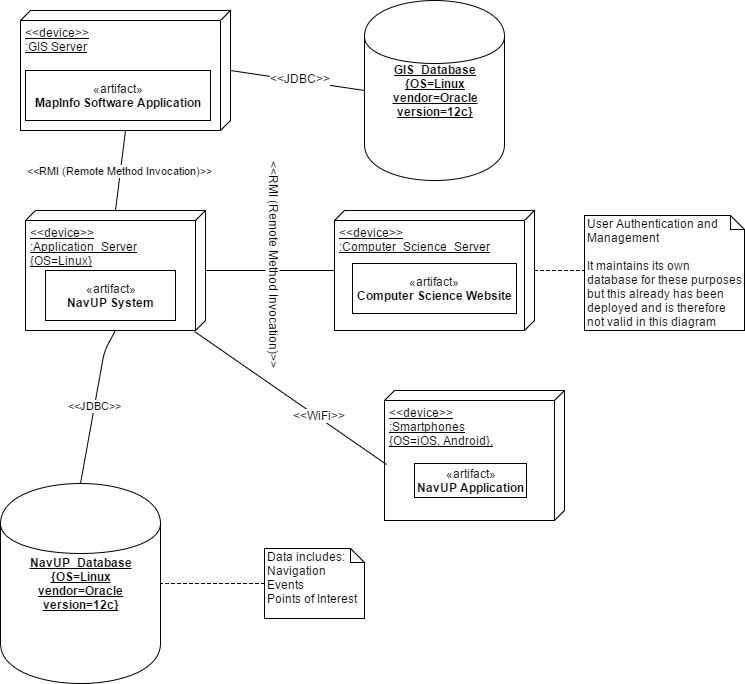
\includegraphics[width=0.7\textwidth]{DeploymentDiagram.jpg}
   	\caption{Deployment Diagram for NavUP}
\end{figure}

\subsubsection{Description of NavUP Architecture}
\noindent NavUP can be described as a mixture of an \textbf{Interactive System and Client-Server System}. The users of NavUP have a make a fixed set of requests (view a location, find a route, maintain user profile, view points of interests etc.) and receive fixed responses from the system (an updated map display). However, the \textbf{Notifications} subsystem displays characteristics of \textbf{Event-Driven Subsystem} as it has no fixed notifcation dispatching.
\\ \\
The overall architectural style applied is hence of \textbf{Client-Server} – \textbf{users (clients)}, by means of access channels (Android, iOS, Web) devices will make \textbf{concurrent requests to the application server} which will respond by making use of other servers like GIS, CS Web Server and associated databases to carry out program logic. The deployment diagram depicts this detail of client-server interaction.

\subsubsection{Techonlogy Choices}
\noindent
There are a variety of technology choices that have been made, some of which are indicated on the deployment diagram. Efforts have been made to use \textbf{commercial off-the-shelf (COTS) parts and products} as far as possible to reduce implementation and testing time and improve reliability of the system. There is \textbf{ease of change and maintenance} as the GIS and CS Server can be updated independently of the application server due to the \textbf{distributed nature of the backend} – the client only interacts with the application server.

\begin {itemize} 
\item \textbf{iOS and Android} are without doubt the most used operating systems of devices held by students, staff and visitors in campus. Another benefit includes making the application easily available to users via the \textbf{Google Play Store and Apple iStore}.

\item The latest stable release of \textbf{MapInfo Pro} is July 2016 and is a robust software that will provide access to locations of campus at \textbf{reliable, with fast throughput and response} times as is necessary to make the user experiences of NavUP special.

\item The \textbf{Linux OS} is more programmer friendly with an easier terminal and more options which will be necessary to implement the Application Server. It is the OS which has been used by all COS 301 students in their undergraduate years in modules like Networking and Operating Systems which make it easier for program development.

\item \textbf{Oracle 12c Database} has been chosen because of the following features: upgradability (the database can be upgraded much easier than its competitors in case NavUP expands in the future); cost-effectiveness and the University of Pretoria can get better Customer Service and Support from Oracle than any other product.

\item \textbf{JDBC (Java Database Connectivity)} is part of the Java Standard Edition platform, from Oracle Corporation and hence will function well with our Oracle 12c database. This also means all programming can be done using the \textbf{Java programming language}.

\end{itemize}

\section{External Interface Requirements}

\subsection{User}
The user system interacts with 2 main entities; the web browser and Mail Systems. 

\begin{itemize}
\item \underline{Web browser} The direct interaction with the user occurs on the web browser when the user enters their credetentials to register/login to the system. Since the front-end web application will require a javascript framework (as do most applications in industry today), it will be a requirement that the system is compatible with Google Chrome or Firefox web browsers. 

\item \underline{Mail Systems} When a user registers onto the NavUP system, their email address will be validated by sending a confirmation link to their email account. So in order for registration to occur, the user needs to have a valid email address. 

\end{itemize}
\subsection{Navigation}
The navigation system communicates to three main entities; the network, the user and the user’s device. There needs to be an interface between each one of these entities to allow communication.

\begin{itemize}
\item \underline{User interface:} 
The user interacts with the navigation system via the GUI. This GUI needs to be flexible enough to function on devices of various sizes and operating systems. The interface must allow the user to have some method of control over the navigation system like choosing destinations, waypoints, routes and changes in these routes. 

\item The navigation system should also communicate to the user by showing information on the screen and through audio. This information includes messages on the screen, the map, locations on the map and the possible routes on the map.

\item Other aspects of the user interface like font, icons and the more visual aspects will be decided upon when the GUI is created.

\item \underline{Device Interface:}
In order to allow communication between the device and the navigation system, an interface needs to be created. The navigation system needs access and information from the device in order to function. This includes access to its hardware like the screen, device memory, connection to Wi-Fi or the internet, the location system and information like the device identity. 

\item The navigation system will be installed on the device along with the application. Being on the device itself will give it the needed access, if permission was granted. 

\item \underline{Network Interface:}
The navigation system functions best with communication between it and the network. This connection is established through the device’s connection. The connection can be to a WI-FI network or the mobile data network. 

\item The interface needs to facilitate exchange of information like location, identity, traffic, route information and aspects that might influence how navigation will take place. These aspects can be events, personal preference or personal information like disabilities. 

\end{itemize}

\subsection{Notification}
The notification system consists of three parts: Software, Hardware and User interface. In order for the notification system to function properly, all three should be able to communicate and work together to perform the required tasks. 

\begin{itemize}

\item \underline{Software Interface:}
The mobile application will connect to the database in order to obtain the users’ information. One such example includes obtaining information regarding the individuals selected notification medium. The mobile application will also connect to the server in order to update information regarding the users email address and mobile number.

\item The server will be connected to the notification plugins, which include email and SMS plugins, as well as the application itself in times when notifications are displayed as a pop-up on the users’ mobile device.

\item \underline{Hardware Interface:}
The user will interact with the mobile device screen in order to set their notification medium preference that is sent and stored on the server. 

\item When there is a notification, the server will then send data packets to the mobile application by making use of sockets. This will cause the mobile device to display the message as well as vibrate or make a sound. 

\item The user will once again interact with the screen on their mobile device in order to view the notification.

\item \underline{User Interface:}
The user will initially interact with the notifications module through the application’s GUI where they will request to be notified about a certain event as well as provide their chosen notification medium. 

\item If the chosen notifications medium is email, the user will receive a generic email with the given notification. The email will provide a description of the notification in its title. If required, the email will provide a link to the relevant website for more information concerning the notification. If the user selected to receive notifications via SMS, a message describing the notification will be sent to each user. Once again, a link will be provided in the SMS for more information concerning the notification as required. If the user decided to receive notifications through the application, a pop-up will appear on the applications’ GUI when there is a notification. 

\end{itemize}

\subsection{Points of Interest}
The points of interest system is controlled by three main entities: User interface, Software Interface and Hardware Interface. In order for the module to properly function, these entities need to communicate with each other via an interface.
\begin{itemize}
\item \underline{User interface:} 
When the user interacts with the points of interest module, it will be via the GUI which displays the map of campus, where all the points of interest to the user will be displayed. The points of interest should be shown to the user in a way to clearly indicate that a certain location has a point of interest, but also not be too large to block the user from viewing other locations' details near the point of interest, especially on devices with small screens. 

\item The points of interest module should communicate with the user by letting their device vibrate or make a sound when a new point of interest has been added/detected near the user's current location.

\item \underline{Software Interface:}
The system should make use of the database of registered points of interest and sync their locations to that of the user's current location as to notify the user when they are in range of a point of interest and give them more information about the point of interest.

\item \underline{Hardware Interface:}
The system can only function if there is an interface for the points of interest module to communicate with other modules and hardware to obtain information like the user's current location via the Wi-Fi network on campus.

\item The device's hardware such as its speakers, vibrator and screen will be used in order to notify the user of a point of interest as well as give the user more information about the point of interest.


\end{itemize}


\section{Performance Requirements}

\subsection{User}

The following describes performance requirements for the user module: 

\begin{itemize}
\item User interface operations should respond within less than 0.2 seconds.

\item Sending the authentication mail upon registration should be an asynchronous method call so as not to deadlock the system while waiting for the user to authenticate. 

\item CRUD operations by the admin on admin interface should be processed in no more than 3 seconds. These changes to particular users should reflect onto the user interface in less than 5 seconds.
\end{itemize}

\subsection{Navigation}
Because this application’s performance relies greatly on the navigation system’s performance, it is of vital importance that the navigation system meets its requirements. 


The Navigation System must have an accuracy radius of 3m to perform accurately indoors.
\begin{itemize}


\item The navigation system must be able to calculate and return the optimal route at a fast and efficient pace. It is of little use to know the best route if it takes too long to calculate the route.

\item In order for the system to calculate the best route, and since the fitness system will use data gathered by the navigation system, it is necessary for the navigation system to be able to calculate distance accurately, and it must be able to pass this information along.

\item The navigation system must be able to retrieve and process the needed information at a fast pace so that it doesn’t take up too much processing power from the processor
\end{itemize}

\subsection{Notification}
\begin{itemize}
\item The system should be able to send out a large number of notifications without any delay (within 5 seconds).
Multiple administrators should be able to add new notifications without failure.
\end{itemize}

\subsection{Points of Interest}
The Point of Interest module of system does not have particularly stringent performance requirements.

\begin{itemize}
\item User interface operations should respond within less than 0.2 seconds.

\item CRUD operations by the admin on admin interface should be processed in no more than 3 seconds. These changes to particular users should reflect onto the user interface in less than 5 seconds.
\end{itemize}

The figures do not take into account the network round-trip which is outside the control of the
system.

\section{Design Constraints}

\subsection{User}
	The design constraints that you would have on the User module are the following:
	\begin{itemize}
		\item Guest users - The system will have very little to nothing information about them so in terms of user experience it will have to be very generic, 					un-personalized. So it will be beneficial if the application is designed in a manner that the user would want to login or create an account.
		\item Users - Users will only be able to sign up if the user has no account linked to his email address only one account per email address.
		\item Authentication - The user will be limited to their authentication level and it will limit the use of the application so the system design must 						constrain the user to their authentication level.    
	\end{itemize}
\subsection{Navigation}

The navigation system is constrained by the device hardware, access to information and the network connection.

\begin{itemize}
\item The hardware has direct influence on the efficiency of the navigation system. Poor hardware will lead to the navigation system working too slowly. Since this application must function effectively on various types of hardware, it is constrained to popular, rather simple hardware that is common amongst students. For example, it has to function fluently on both the newest smartphones and the older versions like the Samsung Galaxy S3.

\item The navigation system’s efficiency is also constrained to its ability to connect and communicate to the WI-FI and mobile networks. Since it uses the internet to get a constant flow of data that is used to navigate. This information includes current location, heat-maps and events. This information is used to determine the best routes.

\item A constraint to the navigation system’s accuracy is the accuracy of the location system (GIS). The navigation system uses the location system to find its own location as well as locations of other buildings and areas on the map. If the location is inaccurate, the navigation system might give incorrect routes. 

\end{itemize}

\subsection{Notification}
The notification module has constraints that limit its ability to function to the best of its ability, these include:

\begin{itemize}
\item The server should be able to hold an ever-increasing number of users mobile numbers as well as email addresses without failure.  

\item The user will require both a mobile number or email address and a mobile device with the application installed.
\end{itemize}

\subsection{Points of Interest}
The constraints of the points of interest module include the following:

\begin{itemize}
\item The database where the details about the points of interest are saved should be designed to ensure that it can handle a lot of entries while also allowing the database to be accessed by multiple devices at the same time.

\item The points of interest module is highly dependent on the accuracy of the locations of the points of interest and therefore the GIS system that is used as well as the navigation module.

\end{itemize}

\begin{itemize}
\item The database that the 

\item The user will require both a mobile number or email address and a mobile device with the application installed.
\end{itemize}

\section{Software System Attributes}

\subsection{User}
\begin{itemize}
	\item \underline{Security:} The users must be authenticated to allow them to use the application. This is a big security requirement to enforce the different 								levels of access the different users have. This must be done securely so no one can manipulate or break the system to gain 								access to features they are not supposed to have access to.

	\item \underline{Availability:} The system cannot go offline since the users will not be able to be authenticated. If users are not authenticated they cannot 								    access most of the features or functionality
	
	\item \underline {Scalability:} The database should be able to hold a large amount of users' information. As to the large amount of students on campus and 							    the staff's information
\end{itemize}

\subsection{Navigation}
\begin{itemize}
\item \underline{Reliability:} 
This navigation system must be able to function in a WI-FI or internet covered environment as well as a non-covered area up to some extent. Every location on campus must be available on the application. 

\item \underline{Security:}
This navigation system should function without releasing any user information to other devices. This navigation system should not access or be used to access any unneeded information on the user’s device. The user should also have a method of control over the information disseminated to the navigation system.

\item \underline{Availability:}
The navigation system must be part of the original application. It should be activated when the user chooses a route to take instead of constantly calculating routes or finding locations. 

\item \underline{Interoperability:}
The navigation system must function on Android, iOS and in a web-browser.

\item \underline{Accuracy:}
The navigation system must be accurate up to 3m to function indoors but can be less accurate outdoors. 
\end{itemize}

\subsection{Notification}
\begin{itemize}

\item \underline {Flexibility:} 
The notifications system should be implemented in such a way that it will allow for the addition of new notification means.

\item \underline {Maintainability:} The notifications module should be implemented in such a way that future development is allowed. To achieve this, developers should write understandable and well documented code.
 
\item \underline {Scalability:} 
The database should be able to hold a large amount of users contact information as well as be able to notify a large amount of users at the same time.

\item \underline {Reliability:} 
The notifications module should ensure that all the users receive their required notifications.

\item \underline {Security:}
The contact information of the users should be kept secure in order to ensure that third parties do not have access to it. This means that only authorised individuals should be able to access the contact information of the users.

\item \underline {Auditability:}
The system should keep track of the sent and requested notifications.

\item \underline {Testability:}
The notification service should be tested as a whole as well as in isolation regularly to ensure that the notification system still works optimally.

\item \underline {Usability:}
The user should be able to clearly see that the pop-up is a notification.

\item \underline {Integrability:}
The system should allow for future expansions.


\end{itemize}
\subsection{Points of Interest}
\begin{itemize}
\item \underline {Flexibility:}
It is important that the system architecture is such that one can easily
add different access channels to the system. With regards to the Point Of Interest Module, a variety of Points of Interest is key even though it should be bounded and relatable to UP. This is particularly important in the context of the proliferation of connected devices in a world transiting to fully embrace the Internet of Things.
Furthermore, persistence architectures and reporting infrastructures are rapidly evolving as can
be seen from the rapid growth of NoSQL databases such as MONGO DB, semantic knowledge repositories and big data stores. This is very important with regards to Point of Interest as it requires flexible variable data types to serve a wide range of interest. Thus in this context it is important that the application functionality is not locked into any specifc persistence technology and that one is able to easily modify the persistence provider and reporting framework.

\item \underline {Maintainability:}
Amongst the most important quality requirements for the system is maintainability. It is required that the system, in particular, Point of Interest Module, should be easy to maintain in the future. This is so that future developers should be able to easily understand the system; developers should be able to easily and relatively quickly change aspects of the functionality the system provides and furthermore add new funcionality (such as book tickets for an event occuring at a users point of interest).
The technologies chosen for the system should be available for a long time. 

\item \underline {Security:}
Firstly the system needs to support only:
\begin{itemize}
\item Authentication against admin in the admin interface.
\item A configurable authorization framework allowing admin to configure the access to any service to the user, in case certain users are also admin but don't work of the same database that they CRUD Points of Interest over. 
\item Authentication against a chosen user repository. 
\end{itemize}

Pertaining to the future the system is expected to also enforce confidentiality through encrypted communication and protection against man-in-the-middle attacks through hashing.

\item \underline {Auditability:}
The system will log all requests and all responses (including exceptions) for all users and administration operations on the point of interest interface provided by the system.
For each request the log should contain an entry with:
\begin{description}
\item[$\bullet$] a log id for the log entry,
\item[$\bullet$] the time/date stamp when the request was made,
\item[$\bullet$] the user Id of the user/admin performing the operation,
\item[$\bullet$] the user/admin operation performed 
\end{description}

For each response the log should contain an entry with:
\begin{description}
\item[$\bullet$] an log id for the log entry,
\item[$\bullet$] the id of the corresponding request entry,
\item[$\bullet$] the time/date stamp when the response is provided
\end{description}
These logs will accessible to both users and the system.

The system should provide only services to extract information from the audit log and will not
allow the audit log to be modified.

\item \underline {Testability:}
The quality requirements like auditability, integrability, performance, scalability, usability and other requirements should be tested.

The Point of Interest service offered by the system must be testable through:
\begin{description}
\item[$\bullet$] automated unit tests testing components from the admin interface and of the user interface in isolation by the utilization of dummy objects, 
\item[$\bullet$] automated integration tests where components are integrated within the actual Point of Interest environment, and
\item[$\bullet$] test where actual beta test users are used. 
\end{description}

In either cases, these functional tests should verify that:
\begin{description}
\item[$\bullet$] the operation is provided if the pre-conditions are met (i.e. that no exception is raised except if one of the pre-conditions for the service is not met),
\item[$\bullet$] that all post-conditions hold true once the operation has been provided.
\end{description} 

\item \underline {Integrability:} 
Widely adopted public standards should be used to access the service operations provided by the Point Of Interest module. This is so the system can be able to easily address future integration requirements. Furthermore, the use case used for Points of Interest should be accessible from external systems to allow further integration.

\item \underline {Scalability:}
The system will initially be implemented to navigate around the UP campus, but it might be necessary in the future to expand it to manage other facilities such as campuses and mall, therefore it should be scalable to such a user per campus or facility.
\item \underline {Usability:}
Users must be able to login, navigate to different locations. Utilize additional features provided by the application and logout without hassle. The interface should not be cluttered and should not contain redundant information. As management of information on the system is critical, accessing said information should be as simple as possible.
\item \underline {Reliability:} 
It is imperative that the system not experience unnecessary downtime (period of in-operation of the system), thus preventing users from navigating on the maps to specified destinations, or altering information on the system. Additionally there should not be frequent errors within normal operating parameters of the system. Thus simple logins (sessions), alterations on the database, from either users or admin, should not cause errors which affect the system as a whole.

\end{itemize}

\section{UML Diagrams for the Chosen Subsystems}

Design Patterns have been integrated and a discussion of their use are made below the respective diagrams.

\subsection{User} 
\subsubsection{User Class Diagram}
\begin{figure}[H]
   	\centering
   	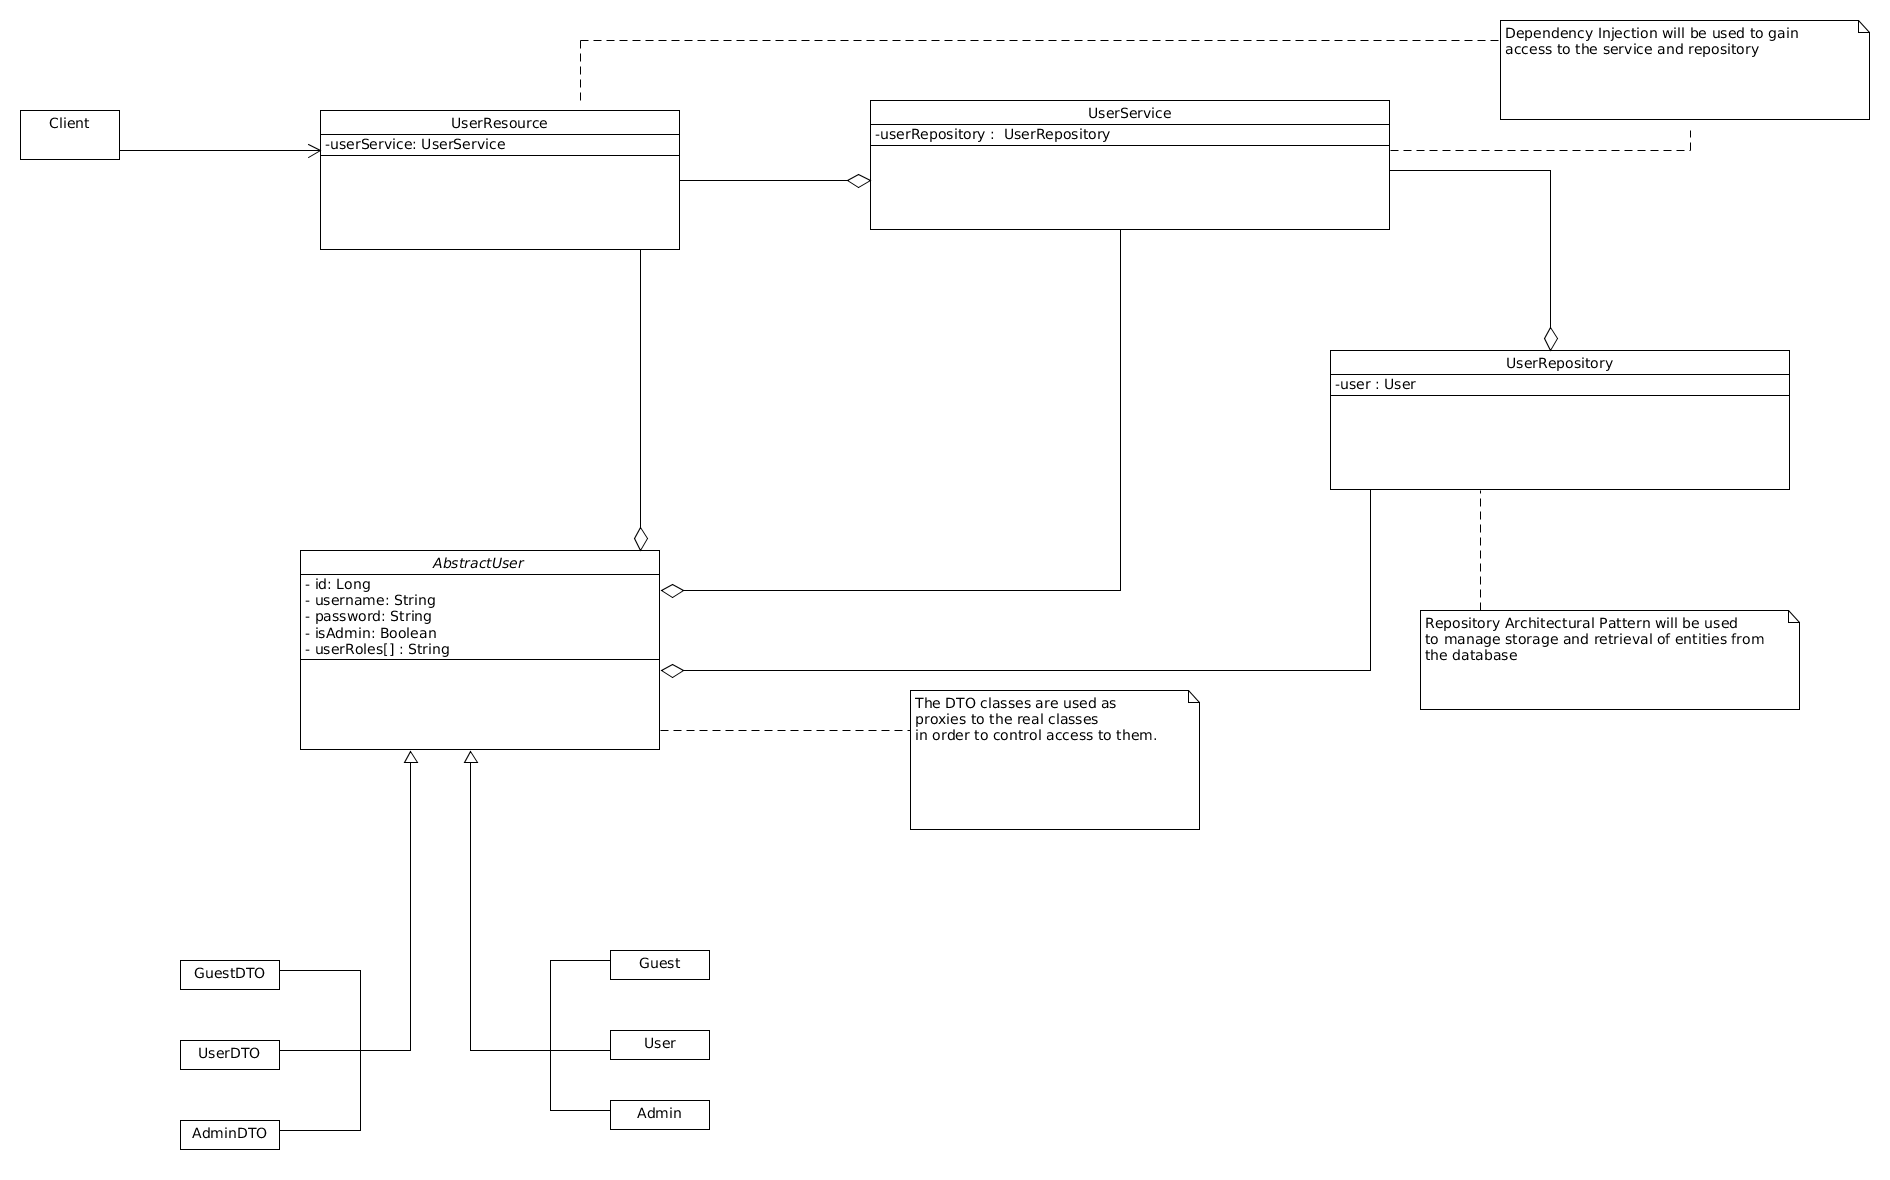
\includegraphics[width=0.7\textwidth]{User_Class_Diagrams.png}
   	\caption{Class Diagram for the User Module}
\end{figure}

\subsubsection{User Use Case Diagram}
\begin{figure}[H]
   	\centering
   	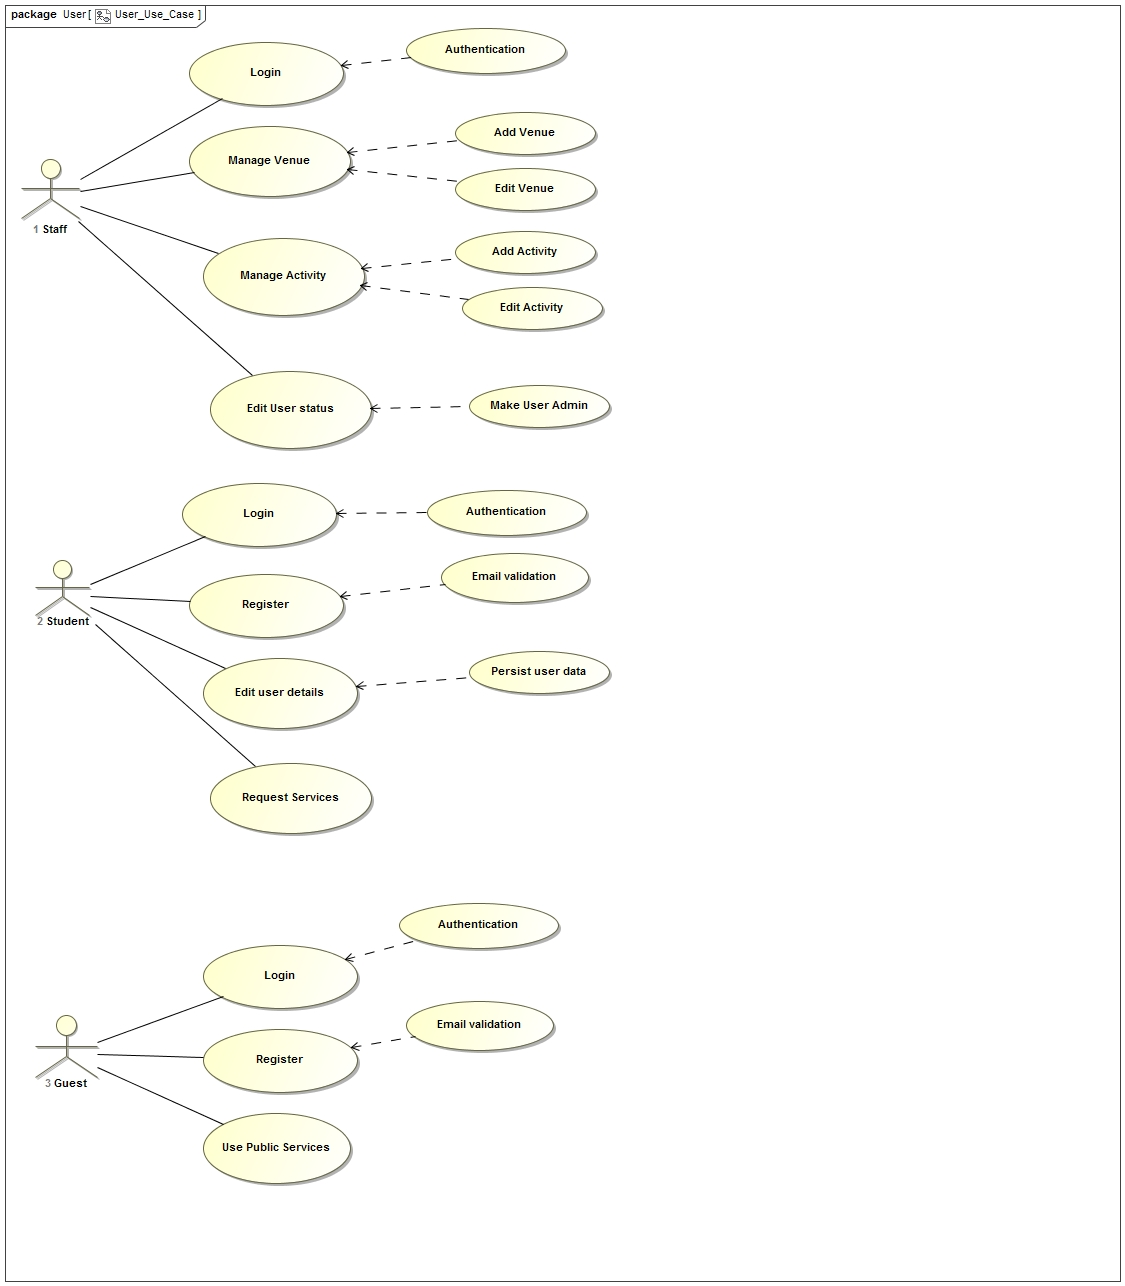
\includegraphics[width=0.7\textwidth]{User_Use_Case.jpg}
   	\caption{Use Case Diagram for the User Module}
\end{figure}

\subsubsection{State Machine Diagram}
\begin{figure}[H]
   	\centering
   	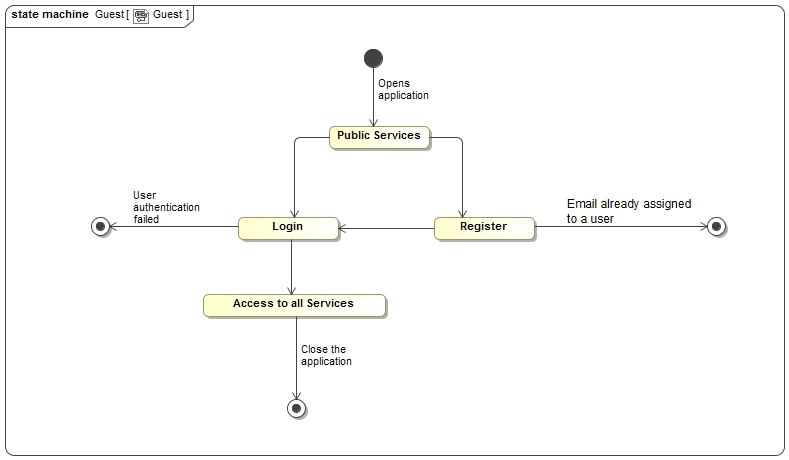
\includegraphics[width=0.7\textwidth]{Guest_State_Diagram.jpg}
   	\caption{State Machine Diagram for the guest in the User Module}
\end{figure}

\subsubsection {Explanation of Design Patterns in User Module}
\begin{itemize}
\item \underline{Proxy Pattern} The Proxy pattern has been used in the users module in order to control access to the user profiles within the backend application. By doing this we add a wrapper and delegation to protect the real component from complexity. 

\item The Data Transfer Objects (DTO's)  can have extra / less fields depending on what the client is or is not allowed to see in the user object. Typically the user object will have more fields than the DTO ( such as roles, hashes of passwords etc). 

\item \underline{Repository Pattern} The Repository Architectural Pattern will be used to manage database access. This pattern enables direct mapping of database objects / row entries to classes. It also delegates the responsibility of managing the database to a single object. Listed below are a few advantages of using the Repository pattern:
	\begin{itemize}
		\item Enables one to maximize the amount of code that can be tested and isolate the data layer to support unit testing. 
		\item Enable one to access the data source from many locations by using dependency injection as well as apply centrally managed, consistent access rules and logic.
		\item Improve maintainability and readability of code by separating business logic from data access logic.  
	\end{itemize} 
\end{itemize}
\subsubsection {Activity Diagram for the User Login Use Case}
 	\begin{figure}[H]
   	\centering
   	\includegraphics[width=0.7\textwidth]{login_activity_diagram.png}
   	\caption{Activity Diagram for the Users Module, Login Use Case}
	\end{figure}
	
	This activity diagram serves to illustrate the flow or actions that will be performed by the system when a user logs onto the system. The getUser() service in the system will be used to retrieve user information to display on the web front-end once a user has been successfully validated and logged in. 
\subsubsection {Sequence Diagram for the User Register Use Case}
 	\begin{figure}[H]
   	\centering
   	\includegraphics[width=0.7\textwidth]{register_sequence_diagram.png}
   	\caption{Sequence Diagram for the Users Module, Register Use Case}
	\end{figure}
	
	The register user use case is described as follows: 
	\begin{itemize}
		\item The user clicks on register on the web browser in order to register their filled in information. 
		\item The web client then creates a REST API call with the POST method to create the user. This request is captured from a REST endpoint in the backend of the application.
		\item When the request is captured in the backend, it is mapped to the userDTO object so that the system can parse the fields in the request body elegantly. 
		\item The userResource then makes use of \textbf{dependency injection} by injecting the UserService into the class. The resource then invokes the createUser() method of the userService. This method will typically expect a UserDTO object to be passed as parameter.
		\item The user service will then instantiate a User object and map the required information from the userDTO to the user object. 
		\item The userRepository service is used in the UserService class via dependecy injection as well. The save() method is invoked which will save the user entry into the database. 
		\item After saving the user details, the repository returns a User object back to the user service. The user service then creates a results userDTO object to return. 
		\item The user object that has been returned from the repository is then mapped to the userDTO that will be returned to the userResource. 
		\item The userResource receives the responseDTO and sends it as a response to the client. This object will be in JSON format. 
	\end{itemize}

\subsection{Navigation}

\begin{figure}[H]
   	\centering
   	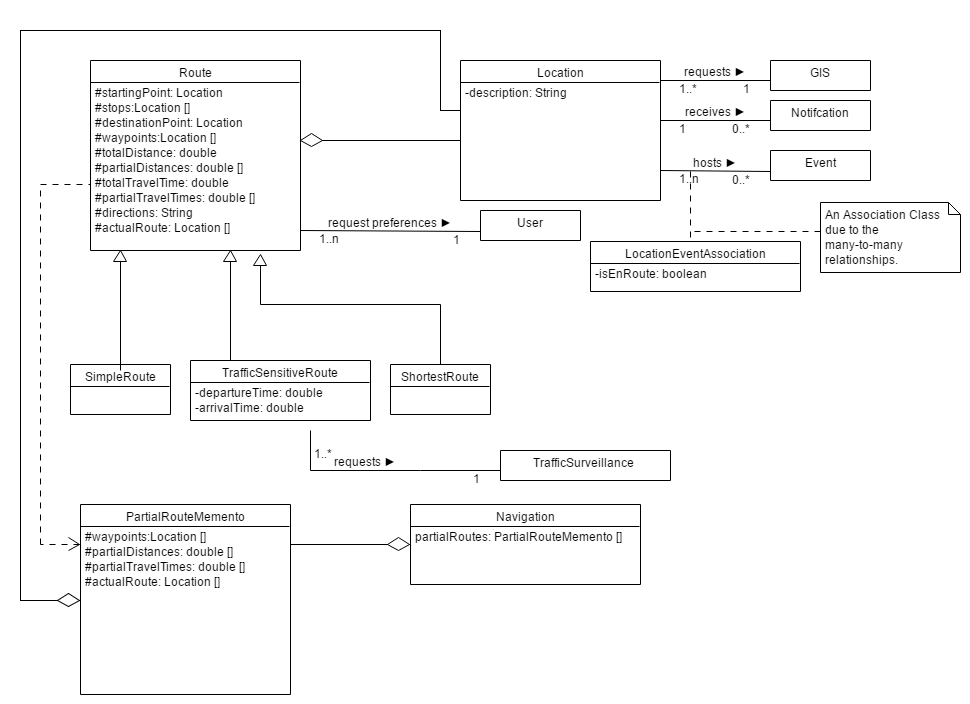
\includegraphics[width=0.7\textwidth]{Navigation-Module-Class-Diagram.png}
   	\caption{Class Diagram for the Navigations Module}
\end{figure}

\subsubsection {Explanation of Design Patterns in Navigation Module}
\begin{itemize}

\item \underline{Memento Pattern} - The Memento Pattern has been used in the navigation module in order to capture the internal state of a "route" object while the route is being calculated.
\item The internal state of the route that we would like to capture is the respective arrays for waypoints, partial distances, partial times and actual distances in the route. 
\item While routing, connection can be lost or the user may diverge from the specified paths during which the system will have to save the internal state so that it can return to this state at a later stage.
\item The role-back function in this case would be the re-route function.
\item The originator in the module is the Route class.
\item The caretaker is the Navigation class.
\item The memento is the PartialRouteMemento class.

\item \underline{Strategy Pattern} - The Strategy Pattern has been used in the navigation module in order to define a family of routing algorithms and make them interchangeable.
\item The users of the system will specify by clicking on different icons, the type of routing they want.
\item The abstraction class would be the Route class which is the interface to the user and is very generic with fundamental functionality.
\item The implementation classes would be the SimpleRoute, ShortestRoute and TrafficSenstiveRoute classes that will override the functionality of the superclass with algorithms for their respective needs.

\end{itemize}

\begin{figure}[H]
   	\centering
   	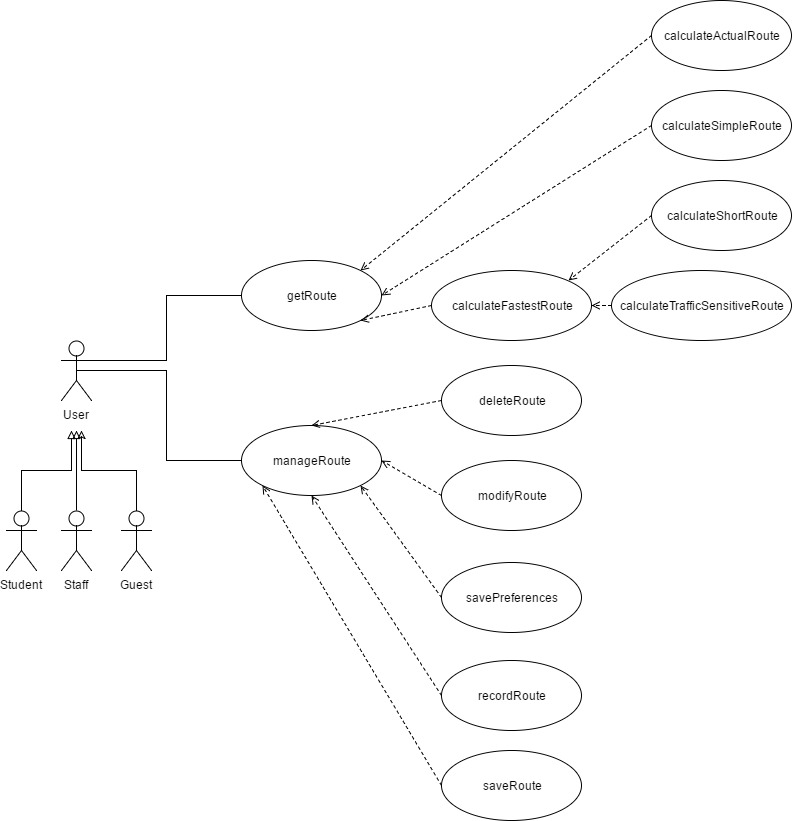
\includegraphics[width=0.7\textwidth]{Navigation-Module-Use-Case.jpg}
   	\caption{Use Case Diagram for the Navigations Module}
\end{figure}


\subsection{Notifications}

\subsubsection{Class Diagram}
\begin{figure}[H]
   	\centering
   	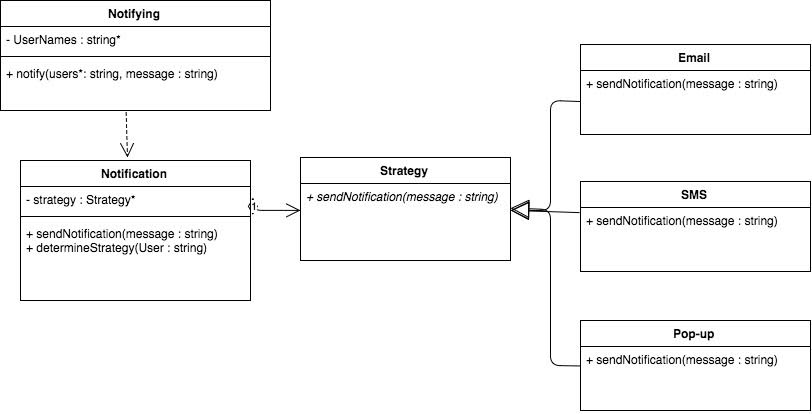
\includegraphics[width=0.7\textwidth]{ClassDiagram.png}
   	\caption{Class Diagram for the Notification Module}
\end{figure}

\subsubsection{Activity Diagram}
\begin{figure}[H]
   	\centering
   	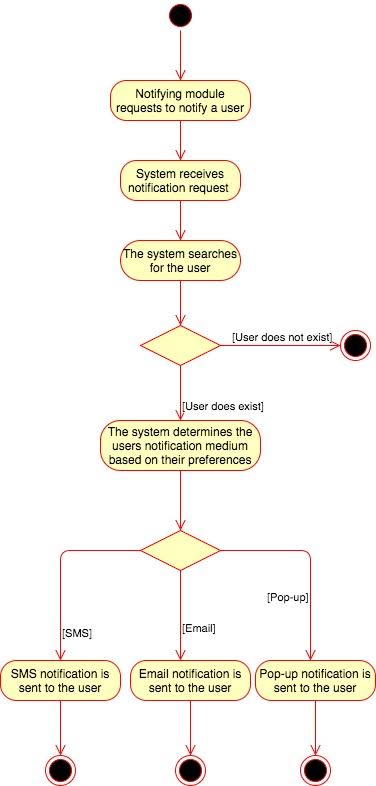
\includegraphics{ActivityDiagram.png}
   	\caption{Activity Diagram for the Notification Module}
\end{figure}

\subsubsection{State Diagram}
\begin{figure}[H]
   	\centering
   	\includegraphics[width=0.7\textwidth]{Notification-StateDiagram.png}
   	\caption{State Diagram for the Notification Module}
\end{figure}

\subsubsection{Use Case Diagram}
\begin{figure}[H]
   	\centering
   	\includegraphics[width=0.7\textwidth]{Notification-UseCaseDiagram.png}
   	\caption{Use Case Diagram for the Notification Module}
\end{figure}

\subsubsection{Explanation of Design Patterns in Notifications Module}
\begin{itemize}
\item \underline{Strategy Pattern} It was used in the notifications module as it will allow for different mediums of communication to be used interchangeably.

The Context participant will be implemented with the Notification class. This class will be responsible for selecting which strategy will be used to notify the individual.

The Strategy in the design pattern will be implemented using the Strategy class. The responsibility of this class will be to call the required notification algorithm.

The Concrete Strategies will include the Email, SMS and Pop-up classes. These classes will responsible for implementing the different algorithms required for notifying the user based on their selected medium.
\end{itemize}


\subsection{Point of Interest}
\begin{figure}[H]
   	\centering
   	\includegraphics[width=0.7\textwidth]{POIClassDiagram.png}
   	\caption{Class Diagram for the Points of Interest Module}
\end{figure}
\subsubsection {Explanation of Design Patterns in Points of Interest Module}
\begin{itemize}
\item \underline{Prototype Pattern} The Prototype pattern has been utilized in this Points of Interest module in ensure Admin creates new Points of Interest working off a certain type.  This makes the creation process easier as they do not need to continuously add information that would be redundant. 

\item \underline{Strategy Pattern} The Strategy Pattern is used to manage the types of Points of Interest accordingly on the User Interface. This ensures that the correct type of Point of interest is accessed accordingly and not making it complex for the controller (The Dashboard) to display the type of Points of Interest. Also it makes it easier for the administration to do requested operations on the right object type.

\item \underline{Observer Pattern} The Observer Pattern exists in this case as it eliminates a potential many to many relationship. The Dashboard provides an interface for the different types of Points of Interest handled by the manager to attach and detach to the Points of Interest Dashboard.

\item \underline{Mediator Pattern} The Mediator is also present as the Dashboard is responsible for controlling and coordinating the interactions of a group of different Points of Interest objects. This pertains to access rights to the user utilizing the dashboard as only the admin have access to certain operations. Class diagram is also structured in such a way that loose coupling exists between the Dashboard and the Points of Interest. Thereby the objects are interacting independently. As the change of states between these the Dashboard and the Points of Interest are independently made. 

\item \underline{Adapter Pattern} The adapter in this case is the Dashboard and the Target for the User and Administration, this is because it contains the Location and so if a different metric unit is required it can call the Adaptee which has operations required to convert and return as a new type.

\item \underline{Flyweight Pattern} As the admin is responsible for the creation and deletion of Points of Interest. In order for dashboard to display (if any) the amount of Points of Interest, a Flyweight is required. This is true as the different Concrete types of Points of Interest are created as soon as the dashboard is accessed  in order to display what types of Points of Interest exists and (if any) the Points of Interest existing.

\end{itemize}
\subsubsection {Activity Diagram for the Points of Interest Module Use Case}
 	\begin{figure}[H]
   	\centering
   	\includegraphics[width=0.7\textwidth]{POI_Activity_Diagram.png}
   	\caption{Activity Diagram for the Points of Interest Use Case}
	\end{figure}
	
	The Point of Interest activity diagram illustrates the progressions of operations that were performed by the system when the user or admin performed operations to the system. 
	 
\subsubsection {Sequence Diagram for the Points of Interest Use Case}
 	\begin{figure}[H]
   	\centering
   	\includegraphics[width=0.7\textwidth]{POISequenceDiagram.png}
   	\caption{Sequence Diagram for the Points of Interest Use Case}
	\end{figure}
	There exists several operations that perform different sequences on the system.
	In the case where the admin adds the Points of Interest to the database it the following occurs:
	\begin{itemize}
		\item  After admin has logged onto system it follows that the admin selects to open the Point of interest component.
		\item Admin then adds Points of Interest given location, which is sent as a request to the location manager to validate location. 
		\item Location admin validates then if true it saves locations onto database.
		\item A promise response JSON is returned to the POI system which checks if Points of Interest have been added onto the POI array, if successful it will return true.
	\end{itemize}
	
	In the case where the user access the Point of Interest and saves it the following occurs:
	\begin{itemize}
		\item  User will open Points of Interest Dashboard, and request to view new open Points of Interest added by the admin. 
		\item The location manager will return the Location Array that will be displayed in coordinates fashion by the map view in the users interface of the dashboard.  
		\item User selects the Points of Interest then sends in request to dashboard to save these locations onto the users database.
		\item Database creates a new object to hold the requested locations to be stored. Once completed the dashboard saves the locations selected onto the database.
	\end{itemize}
	


\section{References}

Kung, D.C. (2013) Object-oriented software engineering: An agile unified methodology. New York: McGraw Hill Higher Education.




\end{document}

